\documentclass[../main/report.tex]{subfiles}
\begin{document}

\chapter{Introduction}
\label{sec:intro}

This report presents the TDT4295 Computer Design Project at NTNU for the fall semester of 2014.

The project is the single task of a course every fall in which a group of students make a working computer from scratch.
This year's group was made out of 9 students from the Computer Science department.
Gunnar Tufte and Yaman Umuroglu, served as advisors for the group throughout the semester and assisted in administrative tasks.

\section{Assignment}

The Computer Design Project's primary tasks include making a custom printed circuitboard (PCB) and  implementing a custom processor architecture on an FPGA.
Together with a microcontroller (MCU) and a choice of I/O components, these will form a complete and working system.
The project is evaluated based on this report and an oral presentation of the work, as well as a prototype demonstration.

The task this year was to create a processor inspired by GPU architectures.
Core requirements included having multiple processor cores and a graphical display output.

\newpage

\subsection{Original Assignment Text}

\vspace{1cm}
\noindent

\begin{quotation}

	\subsubsection{Construct a graphics processing unit (GPU) inspired processor}
    \noindent GPUs play a large role in graphical applications as well as high performance computing.
    They are typically constructed around the SIMD (single instruction multiple data) paradigm and
    include special hardware for accelerating graphics-related operation. The idea is to make a
    GPU-inspired processor architecture that exploits the possibility of parallel computation on a
    single chip. The GPU must be a multi-core system.
    
    \subsubsection{Additional requirements}
    \noindent Your processor will be implemented on an FPGA, and you are free to choose how to
    realize your computer architecture. Studying the architecture of general multicore processors
    and parallel machines options can be a good starting point.\\
    
    \noindent Energy efficiency should be a primary consideration in all phases of the project, from early
    design decisions to how software is written.\\
    
    \noindent The task should also include a suitable application that can produce a graphical output on a
    display to demonstrate the processor.\\
    
    \noindent The unit must utilize a Silicon Labs EFM32 series microcontroller (to act as an I/O processor)
    and a Xilinx FPGA (to implement your architecture on). The budget is 10.000 NOK, which must
    cover components and PCB production. The unit design must adhere to the limits set by the
    course staff at any given time.
\end{quotation}
\newpage

\subsection{A Graphics Accelerator}

The group decided to make the custom GPU inspired processor as an accelerator processor for parallelizable computations.
This means that it would not be designed to run entire programs on its own, but would instead be tasked with particular parallelizable parts of a program.
Its purpose would primarily be to run graphics related operations.
However, it would be programmable with general arithmetic and logic operations, and not have specialized hardware units for performing graphics operations.
It was also decided to send graphical output to screen directly from the accelerator, akin to modern GPUs.
This would form a graphical computer system similar to how modern PCs are organized.

\section{Modern Graphics Processing Units}

% What is a GPU?
% What is its purpose?

Modern GPUs are, in a way, an evolution of former Video Graphics Array (VGA) controllers \cite{gpu_appendix}.
A VGA controller of the early 1990s served as a memory controller and display generator that wrote framebuffer values to a display.
As technology advanced, it received hardware to perform specific graphics related functions.
This eventually evolved into a processor, with its own memory, that incorporated a full set of graphical functions.

A GPU's primary purpose has traditionally been to offload graphical calculations from the CPU and render graphical data to a screen.
Graphical functions are accessed through graphical APIs like DirectX and OpenGL.
Today, GPUs also have general computing capabilities and may serve as co-processors for the CPU in addition to handling their graphical duties.
Non-graphics applications for a GPU include image processing, video encoding, and many scientific computing problems and other large, highly regular calculations.


\subsection{The GPU Market}

% Who makes graphics accelerators?
% For what market do they make these?
% What is performance like for modern GPUs?

% PC market reference:
% http://www.zdnet.com/latest-retail-figures-show-a-stable-pc-market-led-by-apple-and-cheap-notebooks-7000034024/
% NDP provide consumer tracking services. Link: https://www.npd.com/wps/portal/npd/us/about-npd/consumer-panel/
% This is their report: https://www.npd.com/wps/portal/npd/us/news/press-releases/apple-and-chrome-boost-us-retail-pc-back-to-school-sales/


In general, at least one GPU is present in every PC these days, and the market for PCs has been relatively stable for many years \cite{pc_sales}.
These GPUs can take the form of discrete chips or be integrated with the CPU.
Intel, AMD, and NVIDIA are the big actors in the PC GPU market \cite{gpu_overall_sales}.
Intel is largest overall but only makes GPUs integrated with their CPUs.
AMD and NVIDIA share the discrete GPU market \cite{gpu_discrete_sales}.
A big market for the more powerful discrete GPUs is the computer gaming industry.
This market has contributed a great deal to the rapid progression of graphics technologies.
With the advent of general purpose GPUs, scientific computing has also gained an interest in powerful GPUs.

In the past 6 years, the booming market for mobile smart devices has introduced a new arena for GPUs.
Mobile devices are currently outselling workstations, and every new mobile device sold today is shipped with a small-format GPU.
These GPUs are generally integrated in the device's system-on-a-chip (SoC), and have slightly different design considerations than traditional workstation GPUs.
As for everything else that runs on batteries, power consumption is a primary concern in this format.
Traditionally, this is a concern that GPU design has not needed to prioritize.
The mobile GPU format has opened up for other GPU design companies than the three mentioned above.
The three dominant GPU design companies in the SoC market are Qualcomm, ARM, and Imagination Technologies \cite{gpu_mobile_sales}.

% PC GPU market share reference:
% http://jonpeddie.com/news/comments/gpu-shipments-marketwatch-q2-2014-charts-and-images/
% and: http://jonpeddie.com/publications/add-in-board-report/
% SoC market share reference: http://jonpeddie.com/press-releases/details/qualcomm-single-largest-proprietary-gpu-supplier-imagination-technologies-t/
% "Jon Peddie Research (JPR) is a technically oriented computer graphics marketing and management-consulting firm"

\subsection{An Enormous Task}

Producing computer graphics is a highly processing intensive task.
To illustrate why computers and mobile devices include a separate GPU, lets look at some back-of-the-envelope calculations.

Consumers expect their computers to display videos and games in Full HD resolution (1920*1080 pixels), which adds up to about 2 million pixels per frame.
To color one pixel accurately in a 3D environment, the processor typically needs to calculate vectors in 3D space, interpolate texture data, adjust for light intensity, and more.
All of these tasks require several floating point operations.
For an optimistic estimate in a fairly simple scene, assume that the CPU needs to perform LOLSOMANY operations per pixel. \todo{fix some numbers}
In this case, even with a clock speed of 4 GHz and no other interfering work, a Full HD screen will receive an unacceptably low framerate.
Fortunately, pixels can often be computed independently of each other.
CPUs, however, are optimized for single-thread performance and fail to take advantage of this.

\subsection{Taking Advantage of Parallelism}

For a CPU, latency is of primary concern because the next instruction often depends on the result of the previous one.
The CPU needs to complete each instruction as quickly as possible.
This makes the CPU very good at problems with a low level of parallelism, which after all characterizes most programs.
Finishing an instruction as quickly as possible is less of a concern when problems are more parallel in nature.
A GPU therefore optimizes for throughput instead of latency.
It gains throughput by making its architecture highly parallel in all respects.

The fast single-threaded cores in CPUs are replaced with a large quantity of smaller, slower cores.
A GPU gains throughput by spending resources on execution units instead of more cache, prediction logic, or dynamic reordering logic to make one execution unit very effective.
It also exploits parallelism with its deep pipelines, executing many instructions concurrently within each core.
These architectural decisions cause each individual thread to require more wait cycles to wait for memory access or pipeline hazards.
Fortunately, a GPU is not concerned about each individual thread's tardiness, and instead fills these wait cycles by interleaving many threads at once in each core.
Filling every cycle and every pipeline stage with useful work is, of course, essential in optimizing throughput.

% Sophisticated dynamic scheduling schemes works to maximize the utilization of GPU resources.

\subsection{At The Mercy of Memory}

%"Modern GPUs are highly parallel, as shown in Figure C.2.5. For example, the GeForce 8800 can process 32 pixels per clock, at 600 MHz. Each pixel typically requires a color read and write and a depth read and write of a 4-byte pixel. Usually an average of two or three texels of four bytes each are read to generate the pixel’s color. So for a typical case, there is a demand of 28 bytes times 32 pixels = 896 bytes per clock. Clearly the bandwidth demand on the memory system is enormous."

% Some numbers to show amount of memory.
% Graphics workloads demand very high data tranfer rates.

A GPU can deliver very high throughput because of its massive amount of parallelism, but with great computing power comes great memory demand.
Keeping all the computational units in a GPU supplied with enough data is a difficult challenge.
Taking NVIDIA's GeForce 8800 GPU, a top-end model in 2006, as an example, it can process 32 pixels per clock at 600 MHz \cite{gpu_appendix}.
A pixel will usually be 4 bytes in size.
Calculating its value will typically require a read and write of color and depth, and a few texture element reads.
So, on average, there may be a demand of 7 memory accesses of 4 bytes each per pixel.
To sustain this for 32 pixels per clock, this requires up to 896 bytes per clock, or over 537 GB/s, in memory transfers.

To supply the processing units with data, the GPU has to have a complex memory system. 
The memory system uses techniques such as batching memory requests, compression, and different types of memories.
The memory is organized in a hierarchy of memories and caches, of different sizes.
The dram interface for the GeForce 8800 had 384 pins, making a bandwidth of up to 96 GB/s possible.
To further increase the bandwidth compression is used to reduce the amount of data that has to be transmitted.
To increase the memory throughput memory requests are saved up and sent in batches.
This creates a lot of latency for memory requests, which means hiding this latency from the programmer is important.
 
\begin{itemize}
	\item The memory buses are wide.
\end{itemize}


\subsection{Design Considerations}

% What kind of functional requirements does a GPU have?
% What issues are important to deal with when designing a GPU?
% - keeping the memory bus saturated
% - scheduling, to utilize the resources
% - thread divergence(branching)

\section{NVIDIA's Fermi Architecture} % or whatever architecture you want...
%http://www.nvidia.com/content/PDF/fermi_white_papers/P.Glaskowsky_NVIDIAFermi-TheFirstCompleteGPUComputingArchitecture.pdf
%http://www.nvidia.com/content/PDF/fermi_white_papers/NVIDIA_Fermi_Compute_Architecture_Whitepaper.pdf

To get an idea of what an actual modern GPU architecture looks like, an overview of NVIDIA's Fermi architecture is presented.
In addition to some details specific to Fermi, this section introduces central concepts relevant for our architecture, such as \emph{warps}, \emph{kernels} and more.

\todo{Rewrite these two paragraphs to fit together. Also the second paragraphs talk about Tesla, while we are presenting Fermi}


\todo{Move this paragraph up?@}

In 2006 NVIDIA released their first GPUs with a so called \emph{unified shader architecture}.
Before this GPUs had seperate and dedicated hardware for the main graphics operations, 
but with this architecture the major operations are executed on the same hardware.
This is significantly different from earlier GPU microarchitectures, and opened
for the possibility to do other calculations on a GPU than graphics processing.

At the heart of Fermi lies the 16 Streaming Multiprocessors (SMs). 
Each SM contains 32 execution cores that can do integer and floatig point operations, 
along with four special-function units, 16 load store units, 
and 64K of SRAM used for cache and local memory.

To be able to have as many cores as possible, NVIDIA kept them simple by not allowing them to do more advanced functions, such as sin, cos or reciprocal.
Instead, there are special cores for these operations, called special-function units, and they are much fewer.

\begin{figure}[H]
\centering
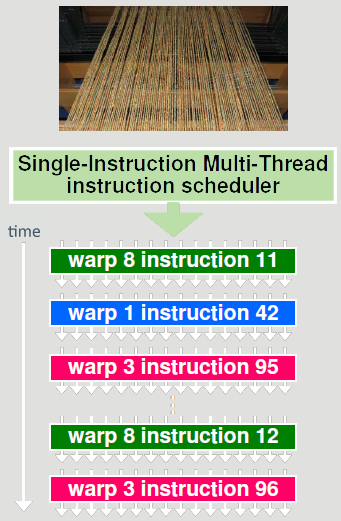
\includegraphics[width=0.4\textwidth]{../introduction/assets/warp.png}
\caption{Warps of 32 threads execute }
\label{fig:simple-nvidia-warps}
\end{figure}


Threads are divided into logical units of 32 threads that are called \emph{warps}. 
The threads in a warp always execute the instruction at the same time.
This way, only a single instruction fetch is required.
A simplified example execution order is shown in figure \ref{fig:simple-nvidia-warps}.
In reality, Fermi executes two instructions per warp per cycle. 
At any point in time there is a set of active warps that are dynamically scheduled. 
A warp is always executed in the same SM, and when it executes an instruction, there is one thread per core, hence 32 cores per SM.



\subsection{CUDA/OpenCL}

To open the powers of the graphics card for other applications, there was a need for a new API that could be
used run code on the GPUs. It has been possible to do non-graphical calculations on GPUs before by 
redifining problems as graphical problems, but this is highly impractical. 
So with the new architecture NVIDIA released a framework for running code on their GPUs called CUDA, 
which let's the programmer run arbitrary code that gains he benefit of the massively parallel hardware.

In order to explain the programming model, we'll jump straight to an example.
Let's say you want to fill a frame buffer, an area of memory, with the color green.
We'll assume that the memory area starts at location 0.
In a sequential programming model one would typically write a loop that would fill
the memory locations with the value for green one by one. 
See listing \ref{sequential-green}.

\begin{c-code}[caption=A sequential program filling the screen with green, label=sequential-green]
int green = 0x00FF00;
for (int i = 0; i < nr_of_pixels; i++){
	framebuffer[i] = green;
}
\end{c-code}

However, in CUDA it is more natural to write a \emph{kernel} that fills only a single pixel with green, 
and then run it with one thread for every pixel.
Below, in listing \ref{lst:green-kernel}, 
you see a CUDA kernel that fills a single memory location, or pixel, with green. 

\begin{c-code}[caption=A CUDA kernel filling a single pixel with green, label=sequential-green]
__global__ void fill_screen(int* framebuffer){
	/* Calculate global id of this thread */
	int global_id = blockIdx.x * blockDim.x + threadIdx.x; 
	int green     = 0x00FF00;
	framebuffer[global_id] = green;
}
\end{c-code}

The \_\_global\_\_ identifier simply tells the CUDA compiler that this is code that can be run on the GPU, or device as it's called in the CUDA terminology.

The function starts, on line 3, by calculating global thread id, a number that is unique for every thread. 
The unique IDs will go from 0 to the total number of threads - 1.
We'll come back to the details of this calculation later.

Line 4 simply stores the hex value for green
, given that values are stored as RGB values with each color consisting of one byte.

Line 5 is where the magic happens. 
It stores the green value to the framebuffer offset by the current thread's ID.
The effect being that thread nr ID colors the pixel nr ID green.

So, how do make this code execute on the device (GPU)?
You have to write code that runs on the host (CPU) which starts the kernel with an appropriate number of threads.

But before we take a look at that, a few words have to be said on how CUDA organizes its threads.
In CUDA, threads are divided into blocks. 
The programmer can decide how many threads there should be in each block, and how many blocks to launch.
Threads within a block can communicate and work tighter than threads across different blocks. 
This is because all threads in block is guaranteed to run on the same SM (Streaming Multiprocessor), and have access to the same shared memory.

For our example, it seems reasonable to have one block correspond to one line on the screen.
Let's assume the screen has a full HD resolution, that is 1920 * 1080 pixels.
Then, one block should contain 1920 threads, and we can launch 1080 blocks.

The CPU, or host as it's called in CUDA, is responsible for starting kernels and deciding how many threads should be run.
Code is written for the host in C and compiled with a special CUDA compiler.
Running code on the device (GPU) is done by a simple function call, as seen in listing \ref{cuda-kernel-launch}

\begin{c-code}[caption=Starting the CUDA kernel with one thread per pixel, label=cuda-kernel-launch]
int* frame_buffer_device = cudaMalloc(@);
fill_screen<<<1080,1920>>>(frame_buffer_device);

int* frame_buffer_host = malloc( sizeof(int) * 1920 * 1080 );
cudaMemCpy(@);
\end{c-code}

The code starts running cudaMalloc, which works like a normal malloc except the memory allocated is located on the device (GPU), and the pointer is thus not valid on the CPU.

The second line is the line that actually runs the kernel. 
The @<<<B,T>>> notation tells the compiler that this function should be run on the device with B blocks of T threads.
So here we run the fill\_screen kernel on the device with 1080 block, each with 1920 threads, which is a little over 2 million threads.
The end result is that our frame buffer is filled with green.

At this point we should mention that CUDA does not have direct access to the actual frame buffers on the graphics card that is displayed on the screen, as one uses other libraries, OpenGL and DirectX, to do graphics operations. 
The reason we are using CUDA instead of those APIs for graphics is that it is closer to how the system we built works.

So for the code presented to make sense, we copy the framebuffer back into memory on the host, through a cudaMemCpy call.
It is now easy to convert this framebuffer to an image.
Which would now be green! 

\todo{How to end this section?}

\todo{Mention what a framebuffer is, first time it is used?}

\todo{Talk about why we don't memory allocate on Demolicious somewhere}


\emph{Maybe give a scientific example with result read back. But only if we show it for Demolicious as well@}


\section{Demolicious}

\textit{Why is the name of our system "Demolicious"?@}
\textit{What approach did we take in making a graphics accelerator?@}
\textit{What trade-offs did we have to make?@}
\textit{What were our concerns?@}
\textit{What kind of numbers did we hope to achieve?@}

The Demolicious design is inspired by modern GPU design, like the one described above.
Modern GPUs are very complex, and have long development cycles.
For the Demolicious system the design had to be greatly simplified.
Because of both time and space constraints, many features that define modern GPUs had to be left out.
There is no branching, and there are no caches because of this.
Modern GPUs have dynamic scheduling to better utilize the resources.
The Demolicious GPU uses barrel processing as a static scheduling scheme, and to hide memory latency.


The project will enter history like a reking ball.@

Her name is Licious. Demo Licious.@

\subsection{Solution Requirements}

\textit{How did we arrive at our list of requirements?@}

\begin{table}[htp]
    \centering
    \begin{tabular}{|p{8cm}|l|}
        \hline
        \textbf{Demolicious Functional Goals}                & \textbf{Priority} \\ \hline
        Demolicious should display graphics on screen                           & HIGH    \\ \hline
        Demolicious should be general purpose                                   & HIGH    \\ \hline
        Demolicious should drive video from GPU module on FPGA                  & MEDIUM  \\ \hline
        Demolicious should handle an output rate of about 30 frames per second  & MEDIUM  \\ \hline
        Demolicious should use HDMI for its graphics output	                    & MEDIUM  \\ \hline
        Demolicious should have an example application in the form of a visual demo displayed on screen & LOW \\ \hline
        Demolicious should have a toolchain to make life easier for programmers & LOW     \\ \hline
    \end{tabular}
    \caption{Goals set for the Demolicious system}
    \label{tab:goals}
\end{table}

\newpage
\section{Structure of the Report}

\todo{Write this!}

\end{document}
